\documentclass{SeminarV2}

\usepackage[latin1]{inputenc}
\usepackage{amssymb,amsmath,array}
\usepackage{graphicx}
\usepackage{placeins}

\usepackage{fancyvrb}
\fvset{tabsize=4}

\usepackage{hyperref}
\usepackage{framed}


\usepackage{listings,color}

\definecolor{verbgray}{gray}{0.9}

\lstnewenvironment{code}{%
    \lstset{backgroundcolor=\color{verbgray},
        frame=single,
        basicstyle=\small \ttfamily,
        framerule=0pt,
        breaklines=true
        }}{}

%\lstset{%
%	language=[LaTeX]TeX,
%	basicstyle=\ttfamily,
%	breaklines=true,
%	columns=fullflexible,
%    showtabs,
%    showstringspaces=true
%}

\newcommand{\shellcmd}[1]{\smallskip\\\indent\indent\texttt{\footnotesize\$ #1}\par\vspace{5pt}}

\newcommand{\mV}{ \texttt{multiVitamin} }


%
\voffset -2 cm \hoffset -2 cm \addtolength{\textwidth}{3cm}
\addtolength{\textheight}{2cm}\addtolength{\leftmargin}{0cm}



\begin{document}
%style file for Seminar manuscripts
\title{User Manual}

%***********************************************************************
% AUTHORS INFORMATION AREA
%***********************************************************************
\author{Clemens Malkawi$^1$, Michel Kreck�$^1$, Maximilian Joas$^1$
%
% Optional short acknowledgment: remove next line if non-needed
%\thanks{This is an optional funding source acknowledgement.}
%
% DO NOT MODIFY THE FOLLOWING '\vspace' ARGUMENT
\vspace{.3cm}\\
%
% Addresses and institutions (remove "1- " in case of a single institution)
University of Leipzig  - Department of Computer Science \\
Augustusplatz 10, 04109 Leipzig  - Germany\\}

%
% Remove the next three lines in case of a single institution

%***********************************************************************
% END OF AUTHORS INFORMATION AREA
%***********************************************************************

\maketitle


\section{multiVitamin}
\mV is a software package which allows users to perform multiple alignments with graphs.
There are two algorithms available for this task. The Bron Kerbosch (BK) \cite{}
and the algorithm originally published by Cordella et al. (VF2) \cite{}. Details on the algorithms can be found in the
theory section.\\
The main function of the package is to align two or more graphs following a binary alignment guide tree containing the "best" alignment procedure. The resulting multiple graph alignment is represented as one single graph itself. Next to this main function, there is also the possibility to show all co-optimals of an alignment between 2 graphs or to view graphical representations of graphs.  
Sounds exciting, so let's get started!

\section{Installation}

Clone the repo from github to [yourDir] with 
\shellcmd{git clone https://github.com/mk36fyvy/multivitamin.git}
Navigate to the directory containing the setup.py file 
\shellcmd{cd [yourDir]/multivitamin/multivitamin}
and type
\shellcmd{pip3 install -e .}
Done, now you can run \mV in the command shell. You can test if the installation was successful by typing
\shellcmd{multiVitamin -h}



\section{Graph Format}

A good first step is to familiarize yourself with the graph format. A graph file is basically a text file, we use the extension '.graph'. It is also used interiorly to identify graph files as such.

The file itself is structured as follows (see below for an example): \\

Every graph consists of nodes and edges. Every node has an id, which is a unique integer (handled as a String internally) for each node. Optionally, nodes can be labelled. The id and label are separated by a semicolon (\texttt{;}) in the '.graph'-file. The edges are two connected nodes and represented by the ids of the two nodes separated by a semicolon.\\

Now, let's walk through the overall structure of the '.graph'-file: 

\begin{itemize}
	\item There is a possibility to insert comment lines by preceding comments with \texttt{//} or writing \texttt{;comment} after the comment. These lines will be ignored by the parser. They can be written anywhere in the first paragraph.
	\item The first line indicates the author of the graph. This line has to start with the word "author" to be recognized by the parser.
	\item The second and third lines show the number of nodes and edges respectively. The parser only sees two consecutive integers at the end of the lines, so it is important that the number of nodes is provided before the number of edges.
	\item The next three lines are booleans that indicate whether the nodes / edges are labelled and if the graph is directed. It is important to stick to the order indicated in the \hyperref[fig:graph_example]{example} below.
	\item The blank line indicates the start of the node section. It is important to choose an integer as node id. The label can contain any symbol, except for \texttt{;}.
	\item The node section is separated from the edge section again by a blank line. If the \texttt{Directed graph} option is set to \texttt{False}, the edges are considered undirected. Internally, every edge's reverse is then added to the graph.  
\end{itemize}

\noindent
Let's look at a small example graph for illustration. The graph has 6 nodes which are all labelled with a 'c' and 6 edges which are not labelled. Your graphs need to have exactly this format to use this package. Especially the blank lines are important. You can find a decent number of further examples at \texttt{multivitamin/graph\_examples}. Now that you are familiar with the graph format, we can take a look at how to use the package.


\begin{framed}
\begin{verbatim} 
//this is a sample graph
AUTHOR: Michel K.
#nodes;6
#edges;6
Nodes labelled;True
Edges labelled;False
Directed graph;False

1;c
2;c
3;c
4;c
5;c
6;c

1;2
1;6
2;3
3;4
4;5
5;6
\end{verbatim}
\end{framed}


\newpage
\section{Main functions}
\subsection{Multiple graph alignment -m}
Consider the basic use without any optional flags for the start. You do not have to be in the directory of the package to use \mV. To get an overview of all the flags you can type
\shellcmd{multiVitamin -h}

If you are experienced with command-line tools the information provided by this command might be sufficient to get you started.\\


\begin{figure}[t!]
\begin{code}
usage: multiVitamin [ -h | -m | -c | -v | -d ] [-a] [-s] [-t] [-g]
for example: multiVitamin -ga VF2 -m g1.graph g2.graph g3.graph

multiVitamin - A multiple alignment tool for graphs

Required arguments (These arguments are mutually exclusive):

-h, --help                  show this help message and exit
-m, --multiple <files...>   provide .graph files for multiple alignment '.' 
                              takes all .graph files in the directory as 
                              arguments
-c, --coopt <files...>      provide 2 graphs which will be aligned.
                              Co-optimals will be saved in ./results
-v, --view <files...>       get a visual representation of the given graphs 
                              in one window. This can get confusing for 
                              large or many graphs. Use -d if you want to 
                              see one window per graph.
-d, --disp-mult <files...>  get a visual representation of the given graphs 
                              in one window per graph.

Optional arguments:

-a, --algorithm <BK|VF2>    indicate an alignment-algorithm (default: BK)
                              Warning: VF2 is only suited if there is true 
                              graph-subgraph isomorphism!
-s, --save-all              save all the graphs produced during the 
                              alignment. The graphs are saved as 
                              "[newick].graph"
-t, --save-shorter          save an additional version of the alignment 
                              graph with much shorter node ids
-g, --save-guide            save the guide tree in Newick-format as 
                              "newick.txt"

\end{code}
\end{figure}


There are three main functions resulting in four mutually exclusive flags. One of them is always required to make multiVitamin work. For starters, we look at the case of a multiple alignment of graphs, which is considered the standard use case. 

Just type:
\shellcmd{mulitVitamin -m <pathToGraphFile1.graph> <pathToGraphFile2.graph> ...}
  
This aligns the given graphs with the default algorithm, which is BK. The resulting terminal output provides all the important information about the alignment. An example output can be found below. 


\begin{figure}
    \begin{code}
Reading graph1.graph from Clemens M., Max. J, Michel K.
Successfully parsed graph1.graph

Reading graph2.graph from Clemens M., Max. J, Michel K.
Successfully parsed graph2.graph


                 _ _   _       _  _                   _       
                | | | (_)     (_)| |                 (_)      
 _ __ ___  _   _| | |_ \ \   / / | |_  __ _ _ __ ___  _ _ __  
| '_ ` _ \| | | | | __| \ \ / / ||  _|/ _` | '_ ` _ \| | '_ \ 
| | | | | | |_| | | |_| |\ V /| || |_| (_| | | | | | | | | | |
|_| |_| |_|\__,_|_|\__|_| \_/ |_| \__|\__,_|_| |_| |_|_|_| |_|

                                                v1.0.0      

Calculating multiple alignment with BK algorithm...

*****************************************************************
*                                                               *
*                          RESULTS                              *
*                                                               *
*****************************************************************

---GRAPH ABBREVIATIONS--------------

gr1	>>	graph1
gr2	>>	graph2


---ALIGNMENT------------------------

*NODES (ID, LABEL, NEIGHBOURS)
gr1:4.gr2:2   'd'   ( gr1:1.gr2:5, gr1:2.gr2:3, gr1:5.gr2:4 )
gr1:1.gr2:5   'a'   ( gr1:2.gr2:3, gr1:5.gr2:4, gr1:4.gr2:2, gr1:3.gr2:6 )
gr1:2.gr2:3   'b'   ( gr1:1.gr2:5, gr1:5.gr2:4, gr1:4.gr2:2, gr1:3.gr2:6 )
gr1:3.gr2:6   'c'   ( gr1:1.gr2:5, gr1:2.gr2:3 )
gr1:5.gr2:4   'e'   ( gr1:1.gr2:5, gr1:2.gr2:3, gr1:4.gr2:2 )

*EDGES (ID, LABEL)
( gr1:2.gr2:3,   gr1:3.gr2:6 )   ''
( gr1:4.gr2:2,   gr1:2.gr2:3 )   ''
( gr1:1.gr2:5,   gr1:3.gr2:6 )   ''
( gr1:1.gr2:5,   gr1:2.gr2:3 )   ''
( gr1:4.gr2:2,   gr1:1.gr2:5 )   ''
( gr1:4.gr2:2,   gr1:5.gr2:4 )   ''
( gr1:1.gr2:5,   gr1:5.gr2:4 )   ''
( gr1:2.gr2:3,   gr1:5.gr2:4 )   ''


---NEWICK TREE----------------------

(graph1,graph2)

********************************************************************

Successfully created the directory /home/micheltower/Documents/multivitamin_project/multivitamin/graph_examples/other/results
All files will be saved here.
Saved graph as gr1-gr2.graph

Saved graph id abbreviations as graph_abbreviations.txt

    \end{code}
\end{figure}

In order to assure the uniqueness of node's IDs in a multiple alignment, every node owns a \texttt{mult\_id} attribute, which comes into play here. First, every graph gets a \textit{unique abbreviation string}. It is built from the first two letters of the graph file name and an index, which is incremented each time, a two letter combination is already taken for the specific multiple alignment. 

In the example,graphs 1 and 2 are called gr1 and gr2 respectively. This abbreviation is used to build the unique node \texttt{mult\_id}s.\\\par

\noindent
Let's look at the first line of the nodes section:  

\begin{code}
gr1:4.gr2:2   'd'   ( gr1:1.gr2:5, gr1:2.gr2:3, gr1:5.gr2:4 )
\end{code}

The node \texttt{gr1:4.gr2:2} originates from the alignment of \textbf{node 4 from graph1} and \textbf{node 2 from graph2}. Note that there is a '\texttt{:}' between the graph and the corresponding original node ID and a '\texttt{.}' between the nodes of different graphs. 

As indicated in the terminal output, what follows written in '' is the label of the node. The label handling during alignment is specified in 
\\\par\indent\texttt{[yourDir]/]multivitamin/multivitamin/utils/modular\_product.py}\\\par
At the moment, if any semantic label checks are needed, you should use the VF2 algorithm. See below for more information.

The neighbours of the node are indicated in parentheses, again indicated by the notation explained above.

The edges section shows the edges as follows: \texttt{node1} and \texttt{node2} are indicated with their \texttt{mult\_id} followed by their label. 

The last section indicates the alignment guide tree in conventional Newick format. \\\par

Naturally, apart from the terminal output, \mV saves the results from the alignment. Every file generated will be saved in the \texttt{./results} folder, with '.' being your current working directory. If the folder is already present, \mV simply adds the files, if not, it creates the directory automatically.\\\par

\noindent
Files that will be created after successful multiple alignment:

\bigskip
\begin{tabular}{rp{0.65\textwidth}}
    \textbf{graph\_abbreviations.txt} & easily parseable text file which indicates the full name and abbreviation couples of the graphs used in the alignment\\\\
    \textbf{$<$g1-g2-...$>$.graph} & the graph resulting from the alignment (in .graph-format). The file contains a comment line indicating the guide tree by which it was obtained\\
\end{tabular}
\bigskip

\noindent
Files that can optionally be created by using flags:

\bigskip
\begin{tabular}{lrp{0.65\textwidth}}
  -s  & \textbf{graph\_abbreviations.txt} & easily parseable text file which indicates the full name and abbreviation couples of the graphs used in the alignment\\\\
 -t  & \textbf{$<$g1-g2-...$>$.graph} & the graph resulting from the alignment (in .graph-format). The file contains a comment line indicating the guide tree by which it was obtained\\\\
-t  & \textbf{$<$g1-g2-...$>$.graph} & the graph resulting from the alignment (in .graph-format). The file contains a comment line indicating the guide tree by which it was obtained\\
\end{tabular}
\bigskip


Additionally to the command line output multiVitamin creates a result folder. This folder contains the aligned graph as .graph file. The first line of the .graph file shows the Newik tree of the mulitple alignment. This file could theoretically be used for further computation with mulitVitamin. The results folder contains also a .txt file of the abbrevations of the graph files. These abbrevations are used to indicate in the alignment which node origins from which graph.\\





\subsection{Graph Alignment with the Vf2}
Let us still consider the basic use case with the required flag -m. This flag can
be combined with all optional flags (see section advanced use). One of those optional
flags is -a which specifies the algorithmn that will be used for the alignent.

In order to use the VF2 algorithmn for the alignent you have to use the flag
-a with  "vf2" as parameter in additon to the specification of the input files. So the command would be
"mulitVitamin -f <pathToGraphFile1.graph> <pathToGraphFile2> <optionalMoreGraphFiles>" -a vf2"
This option is only suited for subgraph graph isomorphisms. So the smaller graph
must always fit entirely in the bigger graph. Despite this restriction the
Vf2 is able to align graphs based on the label of the node ids. So a structural
isomorphism is not enough in this case, but the nodes that could aligned
structurally must also fulfill some kind of semantic condition. This is
usefull to align chemical molecules that are represented as graphs.
This condition can be determined by the user in the custom.py

\subsubsection{Custom.py}
The custom.py file can be found in the multivitamin directory of the root folder.
This file contains a functino the check\_semantics function, which by default
returns always true. The code of the custom.py file looks as follows:
\begin{verbatim}[numbers=left,xleftmargin=5mm]
def check_semantics( n, m ):
    '''This function is used in VF2 algorithm to decide,
    whether aligning to nodes is allowed from the
    label point of view.
    In the sample example below, two nodes will only
    be accepted as a legal matching, if the two
    labels are exactly the same.

    Insert your scoring logic below:'''

#    if n.label == m.label:
#        return True
#    else:
#        return False

    return True

def get_results_dir():
    '''define, where the result files will be saved.
    Default is a dir named 'results' in the current
    working directory'''

    return "/results"
\end{verbatim}

If you untoggle the single comments and out-comment the return True, you get a simple
semantic check that only allows nodes to be aligned that have the same label.
However you can go as crazy as you want with it.\\
Besides the check\_semantics method you can also specify the path where your
results should be saved. Just specify your prefered path as a string as return
value from get\_results\_dir(). Before we jump into the supplemtary clasees, which
you might want to modify for a highly sophisticated check\_semantics function, we
want to take a look at the other flag options.
Note: A change in the supplemtary classes is not recommended.
\section{Advanced Usage}
To make multiVitamin work you need one (exactely one) of the following flags:
-m, -c, -v.\\
The -m option has been discussed in depth in the previous sections. It can be used with
every optional flag.\\
The -v flag allows for graphical representation of our .graph files.
You need to proved a graph file. In most cases this will be the graph of the mulitple
alignent. Use: "multiVitamin -v <file.graph>"
It is not compatible with any of the optional flags.\\
The -c flag works only for exactely two input files.
It gives all the co-optimal alignments of the two given graphs. There exist
cases where two graphs have more can be aligned in different, yet optimal ways.
The -c flag calculates all these cases.
Since -c only works with 2 graphs the Optional flags are not helpful.
Only the -a flag could be used to use the vf2 algorithm. Note lead to high
computation costs.
Let us consider the optional flags now.
If you want to save the guide tree in an extra file use -g.
If you not only want the final multiple alignment graph, but also
all alignments in between use -s. If you have three graphs for example graph1, graph2
and graph3. Let us assume multiVitamin gives us a graph which multiple alignment
is represented by this Newick tree: ((graph1,graph2),graph3). Now you
with the option -s you will also get the alignment of graph1 and graph2 as a graph file.\\

\section{Basic Classes}
In order to implement the Bron Kerbosch and Vf2 algorithm, we used three classes.
A graph class, a node class and a edge class. In general the classes should not be altered
by the user. However for the sophisticated user there may be cases in which he or she
wants to make adjustments to this classes. Therefore we will given a brief
overview of them. Figure 2 shows simple UML diagrams of our base classes. The most important methods and attributes will be explained.
\begin{figure}
    %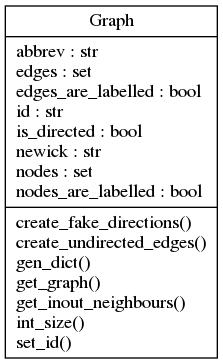
\includegraphics[width=0.5\textwidth]{classes.png}
    %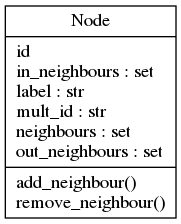
\includegraphics[width=0.5\textwidth]{node.png}
    %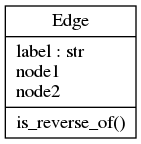
\includegraphics[width=0.5\textwidth]{edge.png}
	{\centering
	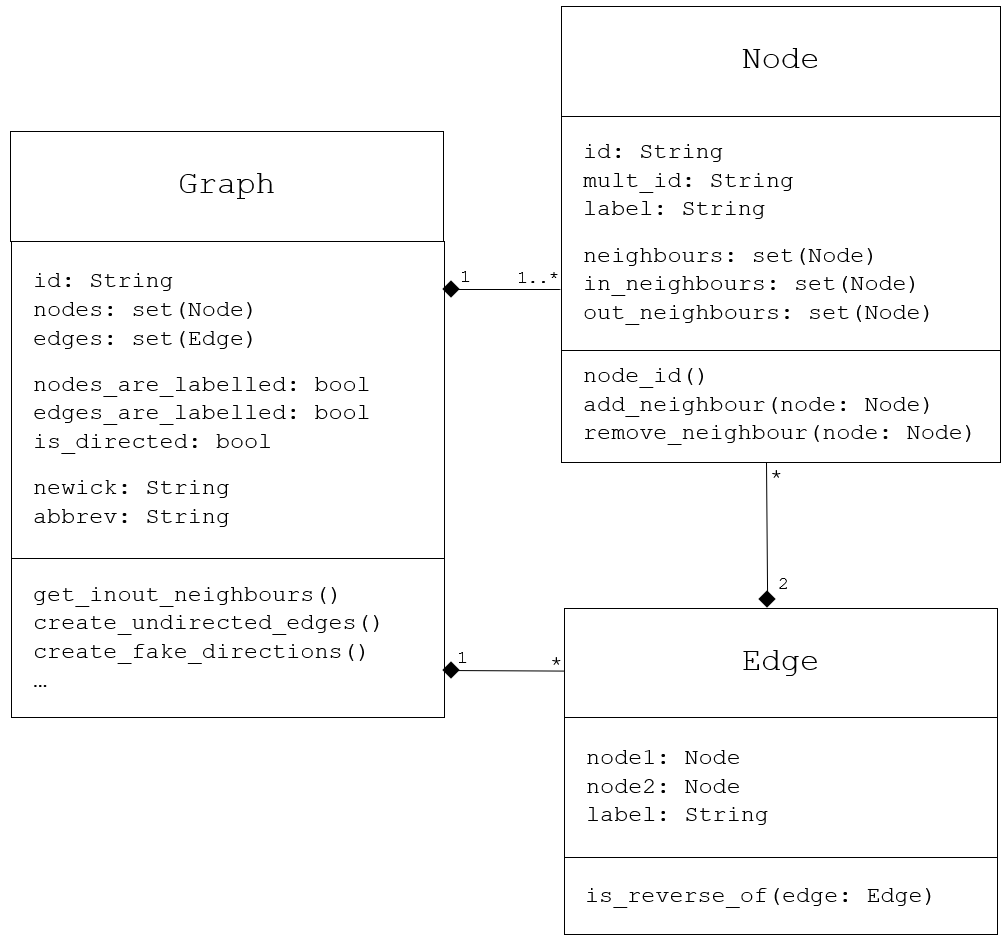
\includegraphics[scale=1.7]{multivitamin_basic_uml.png}
}

  \caption{A UML class diagram of the base classes}
\end{figure}
\subsection{Node}
Our node objects are seen in the context of a graph. Thus every node contains information about
its neighbours. Therefore a node has a neighbours attribute which is a set of Node objects.
In case of directed graphs one can distingush between in and out neighbours. Thus a node object has a seperate set for these two kind of neighbours. This is useful in the Vf2 algorithmn. The mult\_id attribute gives an option to name the node in a mulitple alignment.
\subsubsection{Edge}
An Edge consits of two node objects and an optional label. For each Edge canbe checked if it is the reverse of another edge. This only makes sense for directed graphs.
\subsection{Graph Class}
Besides the obvious attributes of nodes, edges and an id, a graph objects also as an
abbrev which is TODO. Since the Vf2 only works with directed graphs, we 
gave our graphs the possibility to give the graph directions. Consider the Edge A-B. The 
create\_fake\_directions method now points node A to B and node B to A.\\
The method create\_undirected\_edges fills the edge set of the Graph with help of the neighbour set of the node class. The method get\_inout\_neighbours fills the in and outneighbour sets of the node objects in the node set.\\\\
All classes have build in print mehtods for more readable output as well as build in 
methods to compare the objects. So you can determine which graph is larger by the amount of 
nodes in the nodes sets and also determine if two graphs are equal based on their id.\\
Nodes can be also compared by its id and edges by the ids of their nodes.
\section{Theoretical Foundations of the Algorithmns}

\subsection{Bron Kerbosch}
The Bron Kerbosch algorithm solves the problem of finding a maximal common induced subgraphs of two graphs G and H indirectly. This is done by finding the maximal clique in the modular product of G and H s. The set of nodes of the modular product of G and H  is the cartesian N(G) x N(H), with N beeing the set of al vertices of the corresponding graph. Any nodes (u,v) and (x,y), with u,x $\in$ G and v,y $\in$ H in the modular product are adjacemt if:
\begin{itemize}
	\item u and x were neighbours in G and y and x were neighbours in H
	\item u and x were not neighbours in G and y and x were not neighbours in H
\end{itemize}
Before giving two graphs to the Bron Kerbosch to align them we need to build the modular product of these graphs. The rest of our implementaton is straight forward:
\begin{Verbatim}
def bk_pivot ( self, r, p, x ):
	if not any ( [p, x] ):
		self.results.append(r)
		return r
	pivot = self.find_max_pivot( p, x )
	for v in p[:]:
		if  v in pivot.neighbours:
			continue
		r_ = r | {v}
		x_ = x & v.neighbours
		p_ = [n for n in v.neighbours if n in p ]
		self.bk_pivot ( r_, p_, x_ )
		p.remove(v)
		x.add(v)


\end{Verbatim}
The goal of the Bron Kerbosch ,is as mentioned, to find the maximal clique in the modular product. A clique is a subgraph where every node is connected to every other node (=complete graph). A maximal clique is a clique so that no node can added to the subgraph such that the subgraph remains complete.\\
At the beginning r and x are empty sets and theset p that contains all nodes of the modular product of the two input graphs. All nodes in p are candiates for extending the clique.

\subsection{VF2}
\section{Profiling}
To get an idea which algorithm is better sutied for which kind of graph (size, structure),
we did a profiling study. Therefore we used three different kind of graphs:
random graphs, wheel graphs and tree graphs. The graphs where generate with the help of
the python package networkx \cite{}. We did the profiling for the follwoing number of nodes:
(3,8,13,18,23,XX TODO).
In case of the random graphs we created 10 different random graphs for each node count and took the average time per node count. The following figures show the results of our profiling study.





\end{document}

% ****************************************************************************
% BIBLIOGRAPHY AREA
% ****************************************************************************

\begin{footnotesize}
\bibliography{own.bib}
\bibliographystyle{unsrt}
% IF YOU DO NOT USE BIBTEX, USE THE FOLLOWING SAMPLE SCHEME FOR THE REFERENCES
% ----------------------------------------------------------------------------

% ----------------------------------------------------------------------------

% IF YOU USE BIBTEX,
% - DELETE THE TEXT BETWEEN THE TWO ABOVE DASHED LINES
% - UNCOMMENT THE NEXT TWO LINES AND REPLACE 'Name_Of_Your_BibFile'


%\bibliography{Name_Of_Your_BibFile}

\end{footnotesize}

% ****************************************************************************
% END OF BIBLIOGRAPHY AREA
% ****************************************************************************































